\documentclass[twocolumns]{emulateapj}
%apj gives the referee version/preprint2
%\usepackage[T1]{fontenc}
%\usepackage[utf8]{inputenc}
%\usepackage{graphicx}
%\usepackage{natbib}
\usepackage{amsmath}
\usepackage{amssymb}
%\usepackage{vmargin}
%\usepackage{pdfpages}
\usepackage{aas_macros}

\begin{document}
\title{How uniform is TeV-blazar heating?}

\author{A. Lamberts and P. Chang}
\affil{Physics Department, University of Wisconsin-Milwaukee, Milwaukee WI 53211}
\email{lambera@uwm.edu}

%\altaffiltex{1}{Physics Department, UWM, Milwaukee WI 53211}

\begin{abstract}
Write a nice abstract here!


\end{abstract}

\keywords{Best keywords ever}
\section{introduction}
\begin{itemize}
\item modelisation from first principles is impossible. IGM is hard to model and crucial as is is the birthplace for galaxies,
\item Cosmological model
\item Astrophysical interest of TeV blazars
\item inverse ICC but we don't see them, then introduce plasma instabilities (confirmed in recent papers in the non-linear regime)
\item proper modeling of TeV emission crucial for EBL and IGMF
\end{itemize}
\section {Determining the window function}
Our goal is to include additional heating due to TeV blazars in numerical simulations. Determining the formation, evolution and duty cycles of supermassive black holes in numerical simulations at cosmological scales cannot be done in a fully self-consistent manner as the length scales involved are far smaller than the allowed numerical resolution. Therefore, one resorts to subgrid models, which necessarily rely on some parametrization of the underlying physics \citep{}. Although these methods give promising results, we choose instead, to model the heating fluctuations in a more statistical manner. The heating rate can expressed as an mean heating rate plus a small fluctuation
\begin{equation}
  \label{eq:delta_h}
  \dot{q}=\bar{\dot{q}}(1+\delta_H)
\end{equation}

We determine a window function $W_H$, which relates the heating fluctuations $\delta_H$ to the underlying overdensity in a given region $\delta$. The method is based on a Taylor expansion of the quantities describing the TeV sources and keeping only  the first order corrections. This naturally yields the significant lengthscale for heating fluctuations. Our method closely follows the work by   \citet{2007MNRAS.376.1680P,2005ApJ...626....1B}. The detailed computation of the window function, in the Newtonian limit and in an expanding universe, is given in Appendix A. In this section, we present the general method and highlight the underlying hypotheses of our work.

The heating rate at a given point $\vec{x}$ is determined by the received TeV flux from all the sources within a certain radius $r_{max}$ beyond which all the flux gets absorbed. The heating also depends on the rate at which the TeV photons are converted into pairs and that pairs lose their energy to the surrounding medium.  Assuming all the energy of the pairs is converted into heat at the location where they are created \textit{Is this true? How does it change our results if not?}, the heating rate per baryon at a given point is 
\begin{equation}
\label{eq:heating_rate}
  \dot{q}(\vec{x})= \frac{E_0}{4\pi}  \int_{\Omega}\int_0^{r_{max}}   \mathcal{E}(\vec{r}'+\vec{x})\sigma  e^{-\tau}d\Omega dr' ,
\end{equation}
 $E_0$ is the mean energy of the TeV photons and   $\mathcal{E}$ is the emissivity of the sources (photons per unit time, per unit volume). $\sigma$ (in cm$^{-2}$) is the energy averaged cross section for pair production on the extragalactic background light (EBL) and $\tau$ is the associated optical depth along the line of sight. 

One can then express the emissivity as a mean value and a first order correction. The TeV emissivity is related to the presence of a supermassive black holes at centers of galaxys, which are essentially  overdense regions. On average, the larger the overdense region, the higher the TeV emission \textit{any reference about sizes, and the probability for AGN presence?}.  Matter is tightly coupled to the underlying dark matter, which evolution is easy to model analytically as long as linear growth is a valid approximation.  The linear approximation is valid as long as the overdensity is smaller than unity, which is always true in the early universe but then breaks down at small scales as very dense structures form.  Our computation takes into account the bias between baryonic matter and dark matter \citep{1996MNRAS.282..347M}. To model cosmic distances, Eq.~\ref{eq:heating_rate} is integrated in redshift space and we take into account the resulting energy loss for the TeV photons as well as the first order corrections due to proper motions of the sources within the Hubble flow.
\textit{put all the references here or later?}
Switching to Fourier space, Eq.\ref{eq:heating_rate} yields
\begin{eqnarray}
  \label{eq:window}
  \tilde{W}_H(k,z)&=&\frac{1}{\bar{\dot{X}}}\int_{E_{min}}^{E_{max}}dE\int_z^{z_{max}} \\ \nonumber
&&\times \frac{dX(E)}{dz'}\left((b(z)+1)j_0(kr)-\frac{2}{3}j_2(kr)\right)dz', \nonumber
\end{eqnarray}
with 
 \begin{equation}
  \label{eq:define_X}
  X(E,z')=\frac{e^{-\tau(z,z',E)}(1+z')^2}{H(z')\epsilon(E',z')}.
\end{equation}
Assuming the TeV blazar distribution follows the redshift evolution of quasars, \citet{2012ApJ...752...22B} determined the blazar luminosity density in the TeV band based on a fit to \citet{2007ApJ...654..731H}

\begin{eqnarray}
  \label{eq:mean_heat}
  \mathcal{E}(E',z)&=&\mathcal{E}(E',z=0)\Phi_{B}(z)\\ \nonumber
&\simeq& \zeta\epsilon(E',z=0)\Phi_{Q}(z),\nonumber
%&\simeq& \zeta\epsilon(E',z=0)10^{-.0037(1+z)^4+.085(1+z)^3-.0778(1+z)^2+2.795(1+z)-2.133}
\end{eqnarray}
with $\zeta=3.8\times 10^{-3}$ and
\begin{equation}
  \label{eq:phi_quasar}
 \Phi_{Q}(z)=10^{-.0037(1+z)^4+.085(1+z)^3-.0778(1+z)^2+2.795(1+z)-2.133}. 
\end{equation}
 

As the spectra of TeV blazars follow a power law with intrinsic (i.e. redshift corrected) spectral index $\alpha$ , one has

\begin{equation}
  \label{eq:blaz_lum}
  \epsilon(E',z=0)=\epsilon(E_0,z=0)\left(\frac{E'}{E_0}\right)^{-\alpha}\equiv \epsilon_0\left(\frac{E'}{E_0}\right)^{-\alpha},
\end{equation}
with $\epsilon_0=(1.7-4.8)\times 10^{-36}$erg s$^{-1}$ cm$^{-3}=(.5-1.4)\times 10^{38}$ erg s$^{-1}$ Mpc$^{-3}$ the current blazar luminosity. Using 28 TeV blazars, \citet{2012ApJ...752...23C} find that $\alpha\simeq 3$ and $E_0\simeq $ 1 TeV. Following the emission of the nearest TeV blazars, We use $E_{min}=100$ GeV,  and $E_{max}=10$ TeV.

Assuming blazars follow a similar evolution to quasars, we use $z_{maz}=5$  \citep{2007ApJ...654..731H}.

The mean frea path $D_{pp}(E',z)$ of a TeV photon before it interacts with a EBL photon and produces and electron-positron pair  depends on the density of the EBL.  Hence, its redshift evolution is hard to constrain as it is related to the star formation history of the universe as well as its metalicity and dust contents (see e.g \citet{2008A&A...487..837F,2006ApJ...648..774S}).  Following \citet{2012ApJ...752...23C} we use  a prescription 

  \begin{equation}
    \label{eq:mean_free_path}
  D_{pp}(E,z)=35\left(\frac{E}{1 \quad\textrm{TeV}}\right)^{-1} \left(\frac{1+z}{2}\right)^{-\xi} \quad \textrm{Mpc,}   
  \end{equation}

where $\xi=4.5$ for $z<1$ and $\xi=0$ for $z>1$ \citep{2004A&A...413..807K,2009PhRvD..80l3012N}. 

Using Eqs ~\ref{eq:mean_heat} and \ref{eq:mean_free_path} in Eq.~\ref{eq:window} then gives the complete window function for TeV blazar heating as shown of Fig.\ref{fig:window} for $z=0,1,2,3$ and 5. We have computed the window function using an embedded Runge-Kutta method which is able to capture the fast variation of the Bessel functions at large wavenumbers while decreasing computing time at smaller wavenumbers. \textit{Discuss problems at low z, high k?}.

\begin{figure}[h]
  \centering
  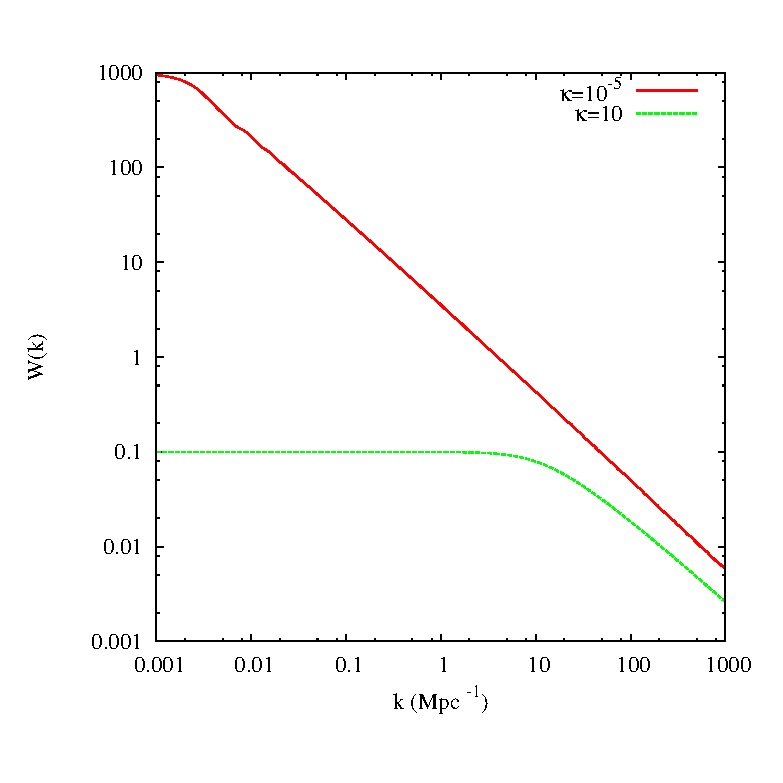
\includegraphics[width = .45\textwidth ]{newtonian_window}
  \caption{Window function for TeV blazar heating from z=5 to the z=0.}
  \label{fig:window}
\end{figure}

\textit{Discuss window function and variation with z}


%is set by all the TeV flux received $J$ by all the sources around $\vec{x}$ and 
 


\section{Numerical method}
\begin{itemize}

\item large mean free path so we have to look at large scales, similar to reionisation problems
\item window function has never been used in simulation
\item resolution effects
\end{itemize}

\section{Results}

\section{Discussion}
\begin{itemize}
\item other heating mechanisms are less efficient
\item heat deposited far from sources. complementary to other feedback mechanisms
\item compare with uniform model
\item suggest possibile applications for window function
\end{itemize}
\section{Conclusions}

\appendix

We detail the derivation of the window function in Eq. \ref{eq:window}. We start from a purely Newtonian universe, then include the impact of expansion and finally the various first order corrections to the received TeV flux.
\section {Newtonian case}\label{sec:windon_newt}

\subsection {Fluctuations with respect to the mean heating rate}

The TeV flux received (in photons s$^{-1}$ cm$^{-2}$) at position $\vec{x}$ is given by the sum over all the sources within a radius $r\leqslant r_{max}$.
\begin{equation}
  \label{eq:flux_recu0}
  J(\vec{x})=\int_{0}^{2\pi}\int_{0}^{\pi}\int_0^{r_{max}}   \frac{\mathcal{E}(\vec{x}') }{4\pi |\vec{x}'-\vec{x}|^2} e^{-\tau} |\vec{x}'-\vec{x}|^2 \sin\theta d\theta d\phi d(\vec{x}'-\vec{x}),
\end{equation}
where the emissivity $\mathcal{E}$ is given in photons per unit time, per unit volume. $\tau=\kappa (\vec{x}'-\vec{x})$ is the optical depth along the line of sight, $\kappa$ the absorption coefficient.
Introducing $\vec{r'}=\vec{x}'-\vec{x}$, and $d\Omega=sin\theta d\theta d\phi$ this gives


\begin{equation}
  \label{eq:flux_recu}
  J(\vec{x})=\int_{\Omega}\int_0^{r_{max}}   \frac{\mathcal{E}(\vec{r}'+\vec{x}) }{4\pi } e^{-\tau} d\Omega dr'.
\end{equation}

The corresponding heating rate (erg cm$^{-3}$ s$^{-1}$ ) is given by 
\begin{equation}
  \label{eq:heating_rate0}
  \dot{Q}(\vec{x})=\frac{E_0}{D_{pp}}J(\vec{x}) =\frac{E}{4\pi}   \int_{\Omega}d\Omega\int_0^{r_{max}}   \mathcal{E}(\vec{r}'+\vec{x}) \frac{1}{D_{pp}}  e^{-\tau} dr' ,
\end{equation}
with $E_0$ the mean energy of the TeV photons and $D_{pp}$ their mean free path  before they pair-produce. For convenience reasons,  we will not take into account the impact of the spectral energy distribution of the TeV photons in this Appendix. It is taken into account in the exact computation in section \S\ref{sec:window}.

This gives the  heating rate per baryon
\begin{equation}
  \label{eq:heating_rate0}
  \dot{q}(\vec{x})=\frac{\dot{Q}}{n}= \frac{E_0}{4\pi}  \int_{\Omega}\int_0^{r_{max}}   \mathcal{E}(\vec{r}'+\vec{x})\sigma  e^{-\tau}d\Omega dr' ,
\end{equation}
where $n$ is the average density of the target photons (i.e. the EBL) and $\sigma$ (in cm$^{-2}$) is the energy averaged cross section for pair production on the extragalactic background light (EBL) photons \citep{1967PhRv..155.1408G}. 


The mean heating rate can be expressed as
\begin{equation}
  \label{eq:heating_rate0}
  \bar{\dot{q}}=\frac{E_0}{4\pi} \int_{\Omega}d\Omega\int_0^{r_{max}}  \bar{\mathcal{E}}\sigma  e^{-\tau}dr', 
\end{equation}
with $\bar{\mathcal{E}}$ the mean emissivity. Throughout the whole appendix, barred quantities are spatially averaged quantities.

The heating rate fluctuations at a given point are then given by 

\begin{eqnarray}
  \label{eq:heat_fluc_newt0}
  \delta_H(\vec{x})&=&\frac{\dot{q}(\vec{x})-\bar{\dot{q}}}{\bar{\dot{q}}}=\frac{E_0}{4\pi\bar{\dot{q}}} \int_{\Omega}d\Omega\int_0^{r_{max}}   (\mathcal{E}(\vec{r}'+\vec{x})-\bar{\mathcal{E}}) \sigma  e^{-\tau} dr' \\ \nonumber
  &=&\frac{E_0}{4\pi\bar{\dot{q}}}\int_{\Omega}d\Omega\int_0^{r_{max}}   \delta_E(\vec{r}'+\vec{x})\bar{\mathcal{E}}\sigma  e^{-\kappa r'}dr',\label{eq:fluc_heat_newt0_b}
\end{eqnarray}
with the fluctuations in the TeV emissivity.
\begin{equation}
  \label{eq:fluc_emissivity}
  \delta_E(\vec{r}'+\vec{x})=\frac{\mathcal{E}(\vec{r'}+\vec{x})-\bar{\mathcal{E}}}{\bar{\mathcal{E}}}.
\end{equation}



\subsection{Window function}
As the universe is infinite and asymptotically flat, we can expand the fluctuations into planar waves, in order to get the lengthscale dependance of heating rate fluctuations \citep{2004MNRAS.352..142B}.

\begin{eqnarray}
  \label{eq:FT_delta}
  \delta_H(\vec{x})&=&\frac{1}{(2\pi)^3}\int_{-\infty}^{\infty} d^3\vec{k'} \tilde{\delta}_H(\vec{k'}) e^{-i\vec{k'}\cdot\vec{x}}\label{eq:FFT}\\
  \delta_E(\vec{r}'+\vec{x})&=&\frac{1}{(2\pi)^3}\int d^3\vec{k'} \tilde{\delta}_E(\vec{k'}) e^{-i\vec{k'}\cdot(\vec{r'}+\vec{x})},
\end{eqnarray}
where the $\tilde{}$ indicates a Fourier transform.
Which gives
\begin{eqnarray}
  \label{eq:heat_fluc_newt1}
\frac{E_0}{(2\pi)^3}\int_{-\infty}^{\infty} d^3\vec{k'} \tilde{\delta}_H(\vec{k'}) e^{-i\vec{k'}\cdot\vec{x}}&=&\frac{1}{4\pi\bar{\dot{q}}_0} \int_{\Omega}d\Omega\int_0^{r_{max}}   \bar{\mathcal{E}}\sigma  e^{-\kappa r'}  \frac{1}{(2\pi)^3}\int d^3\vec{k'} \tilde{\delta}_E(\vec{k'}) e^{-i\vec{k'}\cdot(\vec{r'}+\vec{x})} dr'.
\end{eqnarray}

% To illustrate the next step, we perform a Fourier transform on Eq.\ref{eq:FFT} 
% \begin{eqnarray}
%   \label{eq:left}
% \frac{\tilde(\delta)(k)}{(2\pi)^3}&=&\frac{1}{(2\pi)^3}\int d^3\vec{k'}\tilde{\delta}(\vec{k'}) \int d^3\vec{x} e^{i(\vec{k}-\vec{k}')\cdot \vec{x}} \\
%  &=&  \frac{1}{(2\pi)^3}\int d^3\vec{k}'\delta^{(0)}(\vec{k}-\vec{k}')\tilde{\delta}_H(\vec{k}')\\
%   &=&  \frac{1}{(2\pi)^3} \tilde{\delta}_H(\vec{k})
% \end{eqnarray}




Performing a Fourier transform on the right-hand side of Eq.\ref{eq:heat_fluc_newt0}, we have
\begin{eqnarray}
  \label{eq:right}
  &=& \frac{1}{(2\pi)^3} \frac{E_0}{4\pi\bar{\dot{q}}}\int_{\Omega}d\Omega\int_0^{r_{max}} \bar{ \mathcal{E}}(r')\sigma  e^{-\kappa r'} \int d^3\vec{k'}\int d^3\vec{x} \tilde{\delta}_E(\vec{k'})e^{-i\vec{k'}\cdot{\vec{r}'}} e^{i(\vec{k}-\vec{k'})\cdot\vec{x}}  dr'\\ \nonumber
  &=&\frac{1}{(2\pi)^3} \frac{E_0}{4\pi\bar{\dot{q}}} \int_{\Omega}d\Omega\int_0^{r_{max}}   \bar{\mathcal{E}}(r')\sigma  e^{-\kappa r'} \int d^3\vec{k'} \delta^{0}(\vec{k}-\vec{k}')e^{-i\vec{k'}\cdot{\vec{r}'}} \tilde{\delta}_E(\vec{k'})    dr'\\ \nonumber
  &=&\frac{1}{(2\pi)^3} \frac{E_0}{4\pi\bar{\dot{q}}} \int_{\Omega}d\Omega\int_0^{r_{max}}  \bar{ \mathcal{E}}(r')\sigma  e^{-\kappa r'}  \tilde{\delta}_E(\vec{k}) e^{-i\vec{k}\cdot{\vec{r}'}}  dr',\label{eq:right_3}
\end{eqnarray}
with $\delta^{(0)}$ the Dirac function, which Fourier transform equals 1. Introducing $\mu=cos\theta$, where $\theta$ is the angle between the wavevector and the line of sight, Eq. \ref{eq:heat_fluc_newt0} rewrites
\begin{eqnarray}
  \label{eq:heat_fluc_newt1}
  \tilde{\delta}_H(k)&=&  \frac{E_0}{\bar{2\dot{q}}} \int_{-1}^{1} d\mu \int_0^{r_{max}}  \bar{\mathcal{E}}(r')\sigma  e^{-\kappa r'}  \tilde{\delta}_E(\vec{k}) e^{-ikr'\mu}  dr'\\
&=&\tilde{\delta}_E(\vec{k})\frac{\sigma E_0}{\bar{\dot{q}}}\int_0^{r_{max}} \frac{sin(kr')}{kr'}   \bar{\mathcal{E}}(r')  e^{-\kappa r'}   dr'.\\
&=&\tilde{\delta}_E(\vec{k})\frac{\sigma E_0}{ \bar{\dot{q}}\kappa}  \frac{atan(k)}{k}\\
&=&\tilde{\delta}_E(\vec{k}) \frac{atan(k)}{k}.
\end{eqnarray}

Fig.\ref{fig:window_newt} shows the window function for blazar heating in a purely Newtonian universe.

\begin{figure}[h]
  \centering
  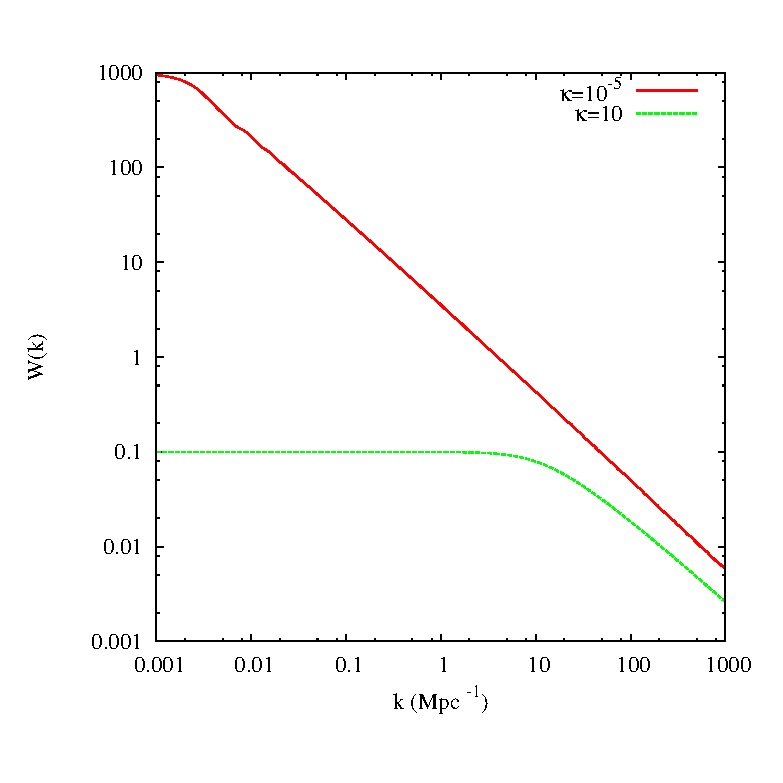
\includegraphics[width = .45\textwidth ]{newtonian_window}
  \caption{Window function for a non-expanding universe.}
  \label{fig:window_newt}
\end{figure}

\textit{Say something. Large regions (small k) of increased emission will result in increased heating rate.  Small scale variations in the emission will not affect the received flux.} 


\section{Expanding universe}\label{sec:window_exp}

We perform the same derivation as in the former section, replacing the integrals on the (proper) distance by redshift integrals using
\begin{equation}
  \label{eq:proper_dist}
  \frac{dr}{dz}=\frac{c}{H(z)}.
\end{equation}
with  $H(z)$ is the Hubble parameter.

 The emissivity $\mathcal{E}$ is given in comoving units, while the heating rate  is expressed in proper units. The proper volume is  $(1+z)^3$ times larger than the comoving volume. 
Let $\vec{s}$ a point with coordinates $(z,\theta,\phi)$, the heating rate at $\vec{s}$ is 

\begin{equation}
  \label{eq:int_exp_heat}
  \dot{q}(\vec{s})=\frac{E_0(1+z)^2}{4\pi}\int_{\Omega}d\Omega\int_z^{z_{max}}\frac{dl}{dz'}\sigma\mathcal{E}(E',z') e^{-\tau} dz'.
\end{equation}
 $z'=z+\Delta z$, with $\Delta z$ the difference in redshift between the emission and reception of the photons.

$\mathcal{E}(E',z')$ is  the   blazar luminosity at the energy $E'$,  which then redshifts to energy $E$ following 
\begin{equation}
  \label{eq:E_z}
  E'=E\frac{1+z'}{1+z}.
\end{equation}

$\tau(E,z',z)$ is the optical depth of a TeV photon observed at redshift $z$ with energy $E$, which was emitted at redshift $z'$ with energy $E'$.

\begin{equation}
  \label{eq:tau}
  \tau(E,z',z)=\int_z^{z'}dz''\frac{1}{D_{pp}}\frac{dl}{dz''}=\int_z^{z'}dz''\frac{c}{H(z)(1+z)}\frac{1}{D_{pp}},
\end{equation}



The mean heating rate is given by 
\begin{equation}
  \label{eq:mean_exp_heat}
  \bar{\dot{q}}=\frac{E_0(1+z)^2}{4\pi}\int_{\Omega}d\Omega\int \frac{dl}{dz'}\sigma\bar{\mathcal{E}} e^{\tau}dz'
\end{equation}
\textit{Here I'm not quite sure about the boundaries for the integral. Should we integrate from z=0 to zmax? I'm also puzzled about what to do with the redshift of the energy.}

The resulting heating rate fluctuations are then given by

\begin{eqnarray}
  \label{eq:heat_fluc_exp0}
  \delta_H(\vec{s})&=&\frac{\dot{q}(\vec{s})-\bar{\dot{q}}}{\bar{\dot{q}}}=\frac{E_0(1+z)^2}{4\pi\bar{\dot{q}}} \int_{\Omega}d\Omega\int_z^{z_{max}} \frac{ ( \mathcal{E}(z')-\bar{\mathcal{E}})c\sigma  e^{-\tau}}{H(z')} dz' \\ \nonumber
  &=&\frac{E_0(1+z)^2}{4\pi\bar{\dot{q}}}  \int_{\Omega}d\Omega\int_0^{z_{max}}   \frac{\delta_E(z')\bar{\mathcal{E}} c\sigma  e^{-\tau}}{H(z')}dz'
\end{eqnarray}

The TeV emission is related to the presence of supermassive black holes at the center of galaxies, which are located in collapsed dark matter haloes.  We can thus connect the fluctuations of the TeV emission, within a certain radius $r$, to the underlying dark matter fluctuations $\delta$, defined by
\begin{equation}
  \label{eq:delta}
  \delta(z,r)=\frac{\rho(z,r)-\bar{\rho}(z)}{\bar{\rho}(z)}
\end{equation}

where $\rho$ is the dark matter  density of the Universe. 

At this stage we will assume the TeV fluctuations exactly match the dark matter fluctuations $\delta_E=\delta$.  We will see in section \ref{sec:total_window} that this is not exactly true and will take into account various corrections.  The initial density fluctuations represent a Gaussian random field, which exact properties depend on the earliest stages of the Universe prior to recombination \citep{1986ApJ...304...15B,Peebles}. Then they grow linearly between $z'$ and $z$ following $\delta(z',r)=\delta_0(r)D(z')/D(z)$ \citep{ 1977MNRAS.179..351H}.

\begin{equation}
  \label{eq:growth_1}
  D(z)=D_0H(z)\int_z^{\infty}\frac{1+z'}{H^3(z')}dz'
\end{equation}
The dark matter fluctuations initially grow linearly as the different Fourier modes of $\delta(\vec{k})$ evolve at the same rate, independently. The linear approximation breaks down when the amplitude of the root mean square of the perturbations approaches unity. The evolution of the density field is then determined by the spherical collapse \citep{1972ApJ...176....1G} and the virialization of haloes.


As the growth of the modes is independent of the wavenumber, we have

\begin{equation}
  \label{eq:FT_delta}
  \delta_E(z',r)=\delta(z',r)=\delta_o(r)D(z')=\delta_0D(z')\frac{1}{(2\pi)^3}\int d^3\vec{k'} \tilde{\delta}(\vec{k'}) e^{-i\vec{k'}\cdot\vec{r}}
\end{equation}


And Eq. \ref{eq:fluc_heat_newt0_b}  rewrites as
\begin{equation}
  \label{eq:heat_fluc_exp0}
  \delta_H(\vec{s})=\frac{E_0(1+z)^2}{4\pi\bar{\dot{q}}} \int_{\Omega}d\Omega\int_z^{z_{max}}  \frac{D(z')}{D(z)} \frac{\delta(r')c \bar{\mathcal{E}} \sigma  e^{-\tau}}{H(z')}dz'
\end{equation}


The left hand side yields $\tilde{\delta}(\vec{k})$ while the right hand side transforms in a similar fashion to Eq. \ref{eq:right_3}. As the power spectrum of density fluctuations is isotropic, this  yields

\begin{equation}
  \label{eq:heat_fluc_exp1}
  \tilde{\delta}_H(k)=\tilde{\delta}(k) \frac{c \sigma \bar{\mathcal{E}}E_0(1+z)^2}{\bar{\dot{q}}} \int_z^{z_{max}} \frac{D(z')}{D(z)}\frac{sin(kr'(z'))}{kr'(z')}    \frac{(1}{H(z')}e^{-\kappa r'(z')}   dz'
\end{equation}

\textit{add plot and explain}

The TeV emission fluctuations are not exactly equal to the DM density fluctuations. In the next section we will account for the various corrections that have to be taken into account to determine a more accurate window function.


\section{Complete window function}

%
\subsection{Galaxy bias}
The TeV flux fluctuations are related to the distribution of galaxies, which is biased with respect to the distribution of DM haloes, which in turn is biased with repect to the initial linear dark matter density fluctuations.  
The formation of galaxies within a certain halo relates to the possibility for the baryonic gas to cool, which is a highly complex astrophysical process. One defines the galaxy bias as the ratio between the power spectrum of galaxies to the power spectrum of the DM haloes (see e.g. \citep{2002PhR...372....1C} for a review).  It is given by
\begin{equation}
  \label{eq:gal_bias}
  b_{gal}=\int_{M_0}^{\infty} dM N(M) b(M) \frac{\langle N_{gal}|M\rangle }{\bar{n}_{gal}},
\end{equation}
where $N(M)$ is the halo mass distribution,  $\langle N_{gal}| M\rangle$ the number of galaxies contained in a halo of mass $M$ and $\bar{n}_{gal}$ the mean number of galaxies per halo. $b(M)$ is the halo bias, relating the halo distribution to the dark matter distribution \citep{1996MNRAS.282..347M}, such that the number of haloes formed in a region of overdensity $\delta$ is given by

  \begin{equation}
    \label{eq:halo_bias}
    N(M,\delta)=[1+b(M)\delta(z)]N(M).
  \end{equation}

$b$ has values of order unity, with increase at higher redshifts. This means that the denser regions of the Gaussian random field are more clustered than the regions with average density. Massive haloes have a stronger bias, as they are not numerous.  In  our computation, the bias is mass-averaged over the halo Press-Schechter halo  mass distribution \citep{1999MNRAS.308..119S}.

 Galaxies bias is usually derived from simulations \citep{1999MNRAS.307..529K}, and observations for low redshifts \citep{2004ApJ...606..702T}. Galaxy bias is only weakly dependent on scale \citep{1998MNRAS.293..209M}, especially at low redshifts. Performing  a fit to Fig.9 in \citet{2004ApJ...601....1W}, we use $b_{gal}(z)=e^{0.4z}$. 


\subsection{Increased area}

 The emitting area (which corresponds to the proper area), is given by
  \begin{equation}
    \label{eq:emitting_area}
A=4\pi r(z)^2=4\pi\left(\frac{\bar{\rho}}{\rho(z)}\right)^{2/3}=4\pi(\delta(z)+1)^{2/3}
  \end{equation}
A small density perturbation thus gives
\begin{equation}
  \label{eq:pert_area}
dA\simeq 4\pi \left(1+\frac{2}{3}\delta\right)
\end{equation}
Note that this is not due to gravitational lensing, which conserves  surface brightness.


\subsection{Redshift-space distortions}
If galaxies were moving exactly with the Hubble flow, their redshift would yield their exact distance to an observer. However, galaxies possess proper random motions with velocity $v$ which cause galaxy clustering to be anistropic in redshift surveys as it changes their redshift, thus the inferred distance. On top off that, galaxies bound to a central potential of a cluster have an infall velocity towards the central overdensity.

%This effect occurs only along the line of sight and does not affect the observed position in the sky, resulting in an elongated structure towards the observer, or ``finger of God''.

 In the linear phase of structure formation, at high redshift, when infall velocities are smaller than the expansion velocity, spherical structures look squeezed towards an observer. Then, at  turnaround, when the infall velocity exactly matches the expansion speed, the galaxy looks like a flat structure. Finally, in the collapsing (non-linear phase), the galaxies look elongated along the line-of-sight. This effect occurs on larger scales than the fingers of God.

Taking into account these corrections,  Eq.\ref{eq:proper_dist} becomes

  \begin{equation}
    \label{eq:vel_perturb}
    dz'=dr\frac{H(z')(1+z')}{c}\left(1-\frac{d\delta_{v_r}(z')}{dr}\right)
  \end{equation}
where $\delta_{v_r}$ are the velocity perturbations along the line of sight.
The Fourier transform of $\delta_{v_r}$ gives  \citep{1987MNRAS.227....1K}.

\begin{equation}
  \label{eq:kaiser2}
  \mathcal{F}\left(\frac{d\delta_{v_r}}{dr}\right)=-\mu^2\tilde{\delta}(\vec{k})
\end{equation}
with $\mu$ the cosine of the angle between the wavenumber and the line of sight.
\textit{verifier delta de r ou de x}

\subsection{Window function }
Keeping only first order correction for density fluctuations, Eq.\ref{eq:int_exp_heat} yields
\begin{equation}
  \label{eq:mean_heat0}
  \dot{q}(\vec{s})=\frac{E_0(1+z)^2c\sigma\mathcal{\bar{E}}}{4\pi}\int_{\Omega}d\Omega\int_z^{z_{max}}\frac{D(z')}{D(z)}\left(1+(b(z)+\frac{2}{3}) \delta(r) -\frac{d\delta_{v_r}}{dr}\right) dz'
\end{equation}

Substracting the mean heating rate (Eq. \ref{eq:mean_exp_heat}) then yields the fluctuations

\begin{equation}
  \label{eq:heat_fluc0}
  \delta_H(\vec{s})=\frac{1}{X}\int_{\Omega}d\Omega\int_z^{z_{max}}\frac{dX}{dz'}\frac{D(z')}{D(z)}\left((b(z)+\frac{2}{3}) \delta(r) -\frac{d\delta_{v_r}}{dr}\right)   dz',
\end{equation}
where we introduced
\begin{equation}
  \label{eq:def_X}
  \frac{dX}{dz'}=\frac{E_0(1+z)^2\mathcal{\bar{E}}c\sigma}{4\pi}\frac{e^{-\tau(z,z',E'}}{H(z')}
\end{equation}
for convenience reasons and to highlight the generality of the method.


Switching to $k$-space then yields


\begin{eqnarray}
  \label{eq:heat_fluc0}
  \tilde{\delta}_H(k)&=&\frac{1}{X}\int_{\Omega}d\Omega\int_z^{z_{max}}\frac{dX}{dz'}\frac{D(z')}{D(z)}\left((b(z)+\frac{2}{3}) \delta(\vec{r'}+\vec{x}) -\frac{d\delta_{v_r}(\vec{r'}+\vec{x})}{dr}\right)  dz'\\
&=&\frac{1}{X}\int_{\Omega}d\Omega\int_z^{z_{max}}\frac{dX}{dz'}\frac{D(z')}{D(z)}\Biggl((b(z)+\frac{2}{3}) \int d^3\tilde{\delta}(\vec{k})'\delta^{(0)}(\vec{k}-\vec{k'})e^{-i\vec{k}' \cdot \vec{r}'}\tilde{\delta}(\vec{k}')- \int d^3\vec{k}'e^{-\vec{k}'\cdot \vec{r}'}\delta(\vec{k}')\delta^{(0)}(\vec{k}+\vec{k}')\mu^2 \Biggr)  dz'\\
&=&\frac{\tilde{\delta}(\vec{k})}{X}\int_{-1}^{1}d\mu\int_z^{z_{max}}\frac{dX}{dz'}\frac{D(z')}{D(z)}\left((b(z)+\frac{2}{3})+\mu^2\right) e^{-ikr\mu}   dz'\\
&=&\frac{\tilde{\delta}(\vec{k})}{X}\int_z^{z_{max}}\frac{dX}{dz'}\frac{D(z')}{D(z)}\left((b(z)+1)j_0(kr)-\frac{2}{3}j_2(kr)\right)dz'
\end{eqnarray}
With the spherical Bessel functions
\begin{eqnarray}
  \label{eq:bessel}
j_0(kr)&=&  \frac{sin(kr)}{kr}\\
j_2(kr)&=& \left(\frac{3}{x^2}-1\right)\frac{sin(x)}{x}-\frac{3 cos(x)}{x^2}  .
\end{eqnarray}
We have used

\begin{equation}
  \label{eq:bes2}
  \int_{-1}^{1}\mu^2 e^{i k r \mu} d\mu=\frac{2 sin(kr)}{kr}+4\frac{cos(kr)}{(kr)^2}-4\frac{sin(kr)}{(kr)^3}
\end{equation}
The window function for the heating rate fluctuations is then given by 

\begin{equation}
  \label{eq:heat_fluc}
  \tilde{W}_H(k,z)=\frac{E_0(1+z)^2\sigma c \mathcal{\bar{E}}}{4\pi\bar{\dot{q}}}\int_z^{z_{max}} \frac{e^{-\tau}}{H(z')}\frac{D(z')}{D(z)}\left((b(z)+1)j_0(kr)-\frac{2}{3}j_2(kr)\right)dz'
\end{equation}

Which is the same window function as  \citep{2007MNRAS.376.1680P,2005ApJ...626....1B}. 



\begin{acknowledgements}
This work was supported by the UWM Research Growth Initiative and NSF grant AST-1255469. Simulations were performed using HPC resources from TACC (Grant TG-AST 130004).\textit{ Did I miss something?}
\end{acknowledgements}

\bibliographystyle{apj}
\bibliography{biblio_total}

 \end{document}
